\documentclass[a4paper]{article}
% Pacotes necessários
\usepackage[portuguese]{babel}
\usepackage[backend=biber, style=apa, citestyle=apa, language=portuguese]{biblatex}
\usepackage{csquotes}
\addbibresource{Recursos/referencias.bib}

\usepackage{amsmath}
\usepackage{graphicx}
\usepackage{subcaption}
\usepackage{setspace}
\usepackage{siunitx} % Required for alignment
\sisetup{
  round-mode          = places, % Rounds numbers
  round-precision     = 2, % to 2 places
}
\usepackage{enumerate}
\usepackage{enumitem}
\usepackage{amsmath}
\usepackage{karnaugh-map}
\usepackage[section]{placeins}
\usepackage{geometry}
\usepackage{amssymb}
\usepackage{titling}
\usepackage[T1]{fontenc}
\usepackage{float}
\usepackage[hidelinks]{hyperref}
\usepackage{xcolor}
\usepackage{indentfirst}
\usepackage{array}
\usepackage{listings}
\usepackage{courier}
\usepackage{soul}
\usepackage{afterpage}
\newcolumntype{P}[1]{>{\centering\arraybackslash}p{#1}}
\onehalfspacing


% Comando para criar uma página vazia
\newcommand\myemptypage{
    \null
    \thispagestyle{empty}
    \addtocounter{page}{-1}
    \newpage
}

% Página de título principal
\newcommand{\firsttitlepage}{
    \begin{titlepage}
        \centering
        
        % Logos superior
        \begin{figure}[h!]
            \centering
            
\includegraphics[width=6cm]{Recursos/Logos/LOGO_IPB.png} % Substitua pelo caminho da imagem
            \vspace{0.5cm}
        \end{figure}

        % Informações da instituição
        \large\textbf{INSTITUTO POLITÉCNICO DE BEJA} \\
        \large\textbf{Escola Superior de Tecnologia e Gestão} \\
        \large\textbf{Mestrado em Engenharia de Segurança Informática} \\
        \large\textbf{Criptografia e Criptanalise Aplicadas} \\
        
        \vspace{2cm}
        
        % Título do projeto
        {\Huge \textbf{Aplicação de Cifra}} \\
        
        \vspace{1.5cm}
        
        % Autores
        \large Martinho José Novo Caeiro - 23917 \\
        \large Paulo António Tavares Abade - 23919 \\

        
        \vfill
        
        % Logo inferior
        \begin{figure}[h!]
            \centering
            
\includegraphics[width=6cm]{Recursos/Logos/IPBejaESTIG.jpg} % Substitua pelo caminho da imagem
        \end{figure}
        
        \vspace{1cm}
        
        % Local e data
        {\large Beja, outubro de 2025}
    \end{titlepage}
}

\newcommand{\secondtitlepage}{
    \begin{titlepage}
        \centering
        \vspace*{1cm}
        
        % Informações da instituição
        \large\textbf{INSTITUTO POLITÉCNICO DE BEJA} \\
        \large\textbf{Escola Superior de Tecnologia e Gestão} \\
        \large\textbf{Mestrado em Engenharia de Segurança Informática} \\
        \large\textbf{Criptografia e Criptanalise Aplicadas} \\
        
        \vspace{2cm}
        
        % Título do projeto
        {\Huge \textbf{Aplicação de Cifra}} \\
        
        \vspace{1.5cm}
        
        % Autores
        \large Martinho José Novo Caeiro - 23917 \\
        \large Paulo António Tavares Abade - 23919 \\

        \vspace{2cm}

        % Orientador
        \large Orientador: Rui Miguel Silva \\
        
        \vfill
        
        % Local e data
        {\large Beja, outubro de 2025}
    \end{titlepage}
}

\begin{document}


\pagenumbering{gobble} % Oculta numeração da página

% Primeira página de título
\firsttitlepage

\secondtitlepage


% Abstract
\section*{\LARGE\textbf{\textit{Resumo}}}

Este relatório descreve o desenvolvimento de uma aplicação de cifra e decifra de ficheiros, implementada em Python,
uma linguagem de alto nível. O objetivo é explorar cifras de criptografia simétrica e demonstrar a aplicação prática das mesmas.
Esta aplicação é desenvolvida no âmbito da unidade curricular de Criptografia e Criptanalise Aplicadas \cite{paglpd}.

\vspace{1cm}
% Keywords
\textbf{Keywords:} python, criptanalise, criptografia simétrica
\newpage
%--------------------------------------------------------------------------------------------------------------------------------------

\section*{\LARGE\textbf{\textit{Abstract}}}

This report describes the development of a file encryption and decryption application, implemented in Python,
a high-level language. The objective is to explore symmetric encryption ciphers and demonstrate their practical application.
This application is developed within the scope of the course Cryptography and Applied Cryptanalysis \cite{paglpd}.

\vspace{1cm}
% Keywords
\textbf{Keywords:} python, cryptanalysis, symmetric cryptography


\renewcommand{\contentsname}{Índice}       % Título do sumário
\renewcommand{\listfigurename}{Índice de Figuras} % Título da lista de figuras

% Início do conteúdo do relatório
\newpage
\doublespacing
\tableofcontents
\listoffigures
\doublespacing

\newpage
\pagenumbering{arabic}

\section{Introdução}\label{intro}
Esta aplicação consistirá na junção de 4 cifras de criptografia simétrica, AES, DES, Vigenère e PlayFair.
A aplicação será desenvolvida em Python (\cite{python}) e tem como base uma interface gráfica simples (GUI),
permitindo ao utilizador interagir com o sistema de forma simples e eficiente.
Todo o progresso do projeto será documentado no repositório GitHub (\cite{github}).

%---------------------------------------------------------------------------------------------------------------------------
\newpage
\section{Introdução Teórica}\label{theory}
\subsection{AES}
O AES (Advanced Encryption Standard) (\cite{aes}) é um padrão de criptografia simétrica amplamente utilizado para proteger dados.
Ele utiliza blocos de 128 bits e chaves de 128, 192 ou 256 bits, oferecendo alta segurança e eficiência.

\subsection{DES}
O DES (Data Encryption Standard) (\cite{des}) é um algoritmo de criptografia simétrica que foi amplamente utilizado no passado.
Ele opera em blocos de 64 bits e utiliza uma chave de 56 bits.
Embora tenha sido substituído por algoritmos mais seguros, o DES ainda é relevante para fins educacionais.

\subsection{Vigenère}
A cifra de Vigenère (\cite{vigenere}) é um método de criptografia que utiliza uma palavra-chave para cifrar o texto.
Ela é baseada na cifra de César, mas em vez de usar um único deslocamento, ela aplica deslocamentos diferentes com
base nas letras da palavra-chave.

\subsection{PlayFair}
A cifra de PlayFair (\cite{playfair}) é um método de criptografia que utiliza uma matriz de 5x5 para cifrar pares de letras.
Ela é mais segura do que a cifra de César, pois não utiliza um deslocamento fixo.

%---------------------------------------------------------------------------------------------------------------------------
\newpage
\section{Desenvolvimento da Aplicação}\label{dev}
Todos os seguintes scripts foram desenvolvidos em Python com o uso do VS Code (\cite{vscode}) e todos verificam se a maquina possui os pacotes necessários
para o funcionamento da ferramenta, irá perguntar se quer instalar para poder continuar a utilizar. Caso
o utilizador deseje prosseguir, o script irá instalar os pacotes necessários e depois irá ativá-los.

%---------------------------------------------------------------------------------------------------------------------------
\subsection{GUI}
A GUI é o metodo principal de interação com a ferramenta. Para aceder a um dos metodos de cifra/decifra, o utilizador deve selecionar a aba correspondente.
Para executar a GUI apenas é necessário escrever `python gui.py`.\\

A GUI apresenta-se da seguinte forma:\\
\begin{figure}[H]
	\centering
	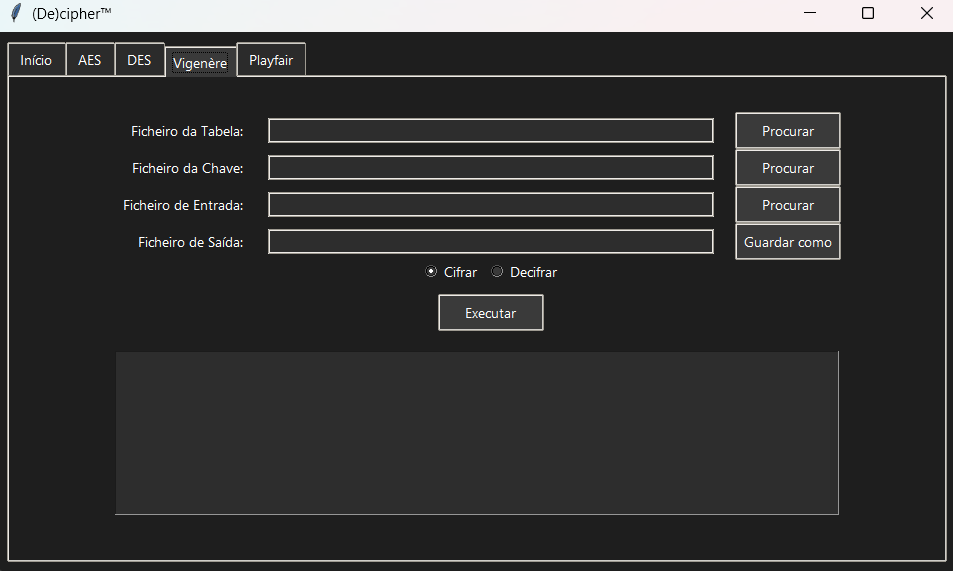
\includegraphics[width=0.9\textwidth]{Recursos/GUI.png}
	\caption{Exemplo da interface gráfica da aplicação.}
	\label{fig:gui_main}
\end{figure}

%---------------------------------------------------------------------------------------------------------------------------
\newpage
\subsection{AES}
Implementou-se uma ferramenta para cifragem e decifragem de ficheiros utilizando AES em modo CBC (biblioteca PyCryptodome).
A chave é carregada a partir de ficheiro através da rotina interna \texttt{\_read\_key\_file}. Essa rotina aceita uma string hexadecimal
(preferencial) ou texto UTF‑8, converte para \texttt{bytes} e valida o comprimento (16, 24 ou 32 bytes). O formato do ficheiro cifrado utilizado
pelo módulo é IV (16 bytes) concatenado com o ciphertext. A encriptação aplica preenchimento compatível com PKCS\#7 para completar blocos de 16 bytes;
a descifragem valida e remove esse preenchimento. Em caso de ficheiro de chave inexistente, tamanho de chave inválido ou padding inválido, são lançadas exceções apropriadas.\\\\

\begin{figure}[H]
	\centering
	\begin{subfigure}[b]{0.48\textwidth}
		\centering
		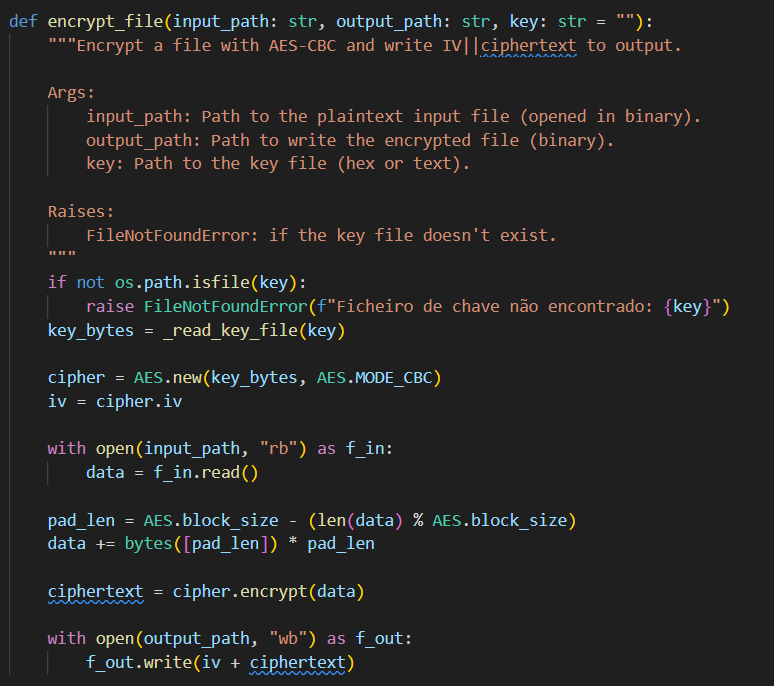
\includegraphics[width=\textwidth]{Recursos/aes_enc.png}
		\caption{Cifragem}
		\label{fig:aes_enc}
	\end{subfigure}
	\hfill
	\begin{subfigure}[b]{0.48\textwidth}
		\centering
		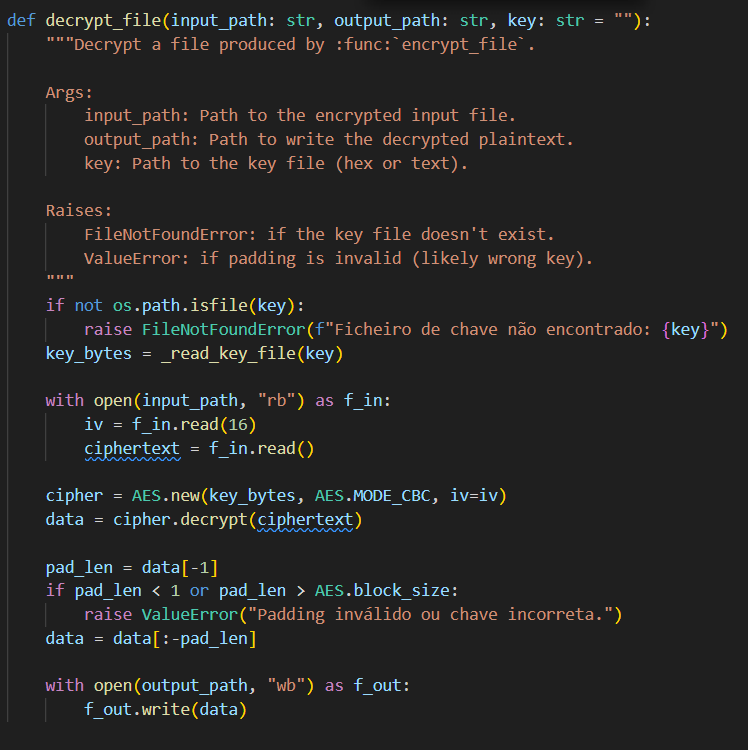
\includegraphics[width=\textwidth]{Recursos/aes_dec.png}
		\caption{Decifragem}
		\label{fig:aes_dec}
	\end{subfigure}
	\caption{AES em modo CBC.}
	\label{fig:aes_combined}
\end{figure}

%---------------------------------------------------------------------------------------------------------------------------
\newpage
\subsection{DES}
Implementou‑se uma ferramenta para cifragem e decifragem de ficheiros utilizando DES em modo CBC (biblioteca PyCryptodome).
A chave é carregada a partir de ficheiro pela rotina interna \texttt{\_read\_key\_file}, que aceita uma string hexadecimal (preferencial)
ou texto UTF‑8, converte para \texttt{bytes} e valida o comprimento (exatamente 8 bytes). O formato do ficheiro cifrado é IV (8 bytes) concatenado com o ciphertext.
A encriptação aplica preenchimento compatível com PKCS\#5 (blocos de 8 bytes); a descifragem valida e remove esse preenchimento. Em caso de ficheiro de chave inexistente,
tamanho de chave inválido ou padding inválido, são lançadas exceções apropriadas.\\\\

\begin{figure}[H]
	\centering
	\begin{subfigure}[b]{0.48\textwidth}
		\centering
		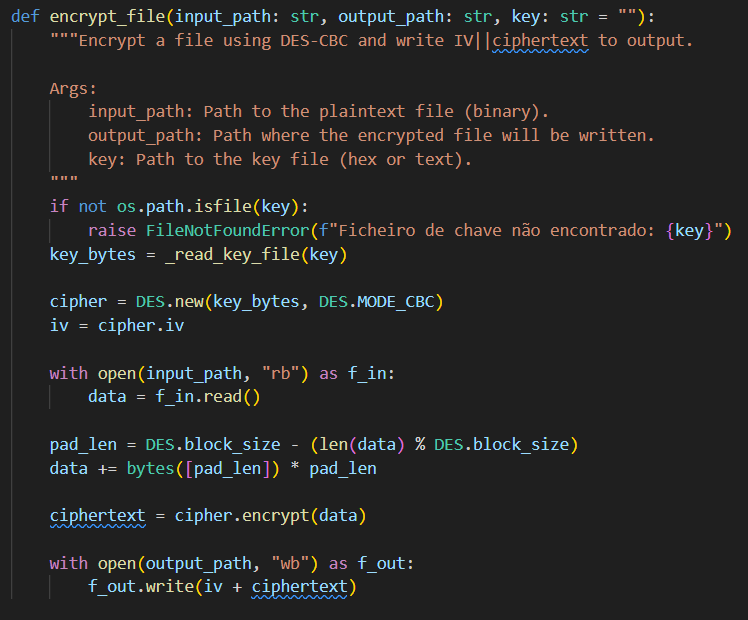
\includegraphics[width=\textwidth]{Recursos/des_enc.png}
		\caption{Cifragem}
		\label{fig:des_enc}
	\end{subfigure}
	\hfill
	\begin{subfigure}[b]{0.48\textwidth}
		\centering
		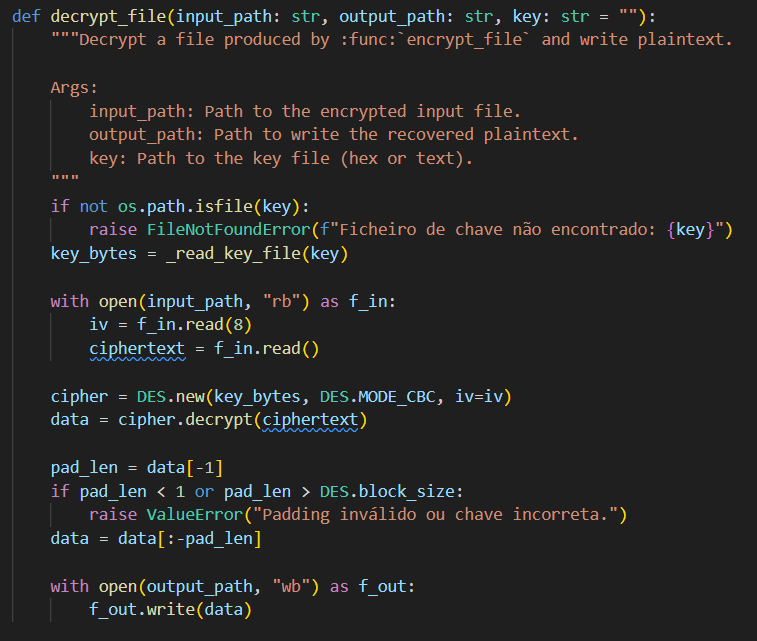
\includegraphics[width=\textwidth]{Recursos/des_dec.png}
		\caption{Decifragem}
		\label{fig:des_dec}
	\end{subfigure}
	\caption{DES em modo CBC.}
	\label{fig:des_combined}
\end{figure}
%---------------------------------------------------------------------------------------------------------------------------
\newpage
\subsection{Vigenère}
Implementou‑se uma ferramenta para cifragem e decifragem de ficheiros usando a cifra de Vigenère com base numa tabela 26×26 carregada através de um ficheiro.
A rotina interna \texttt{read\_table\_from\_file} lê e valida uma tabela com 26 linhas de 26 letras (A–Z);
\texttt{read\_key\_from\_file} lê a chave, filtra apenas letras A–Z e devolve uma string em maiúsculas (valida que não esteja vazia).
O texto é normalizado para letras ASCII visíveis em maiúsculas antes do processamento;
a função \texttt{process\_text} avança o índice da chave apenas sobre letras e usa \texttt{encrypt\_char}/\texttt{decrypt\_char} para cifrar/decifrar carácter a carácter segundo a
linha da tabela definida pelo carácter da chave. As funções \texttt{encrypt\_file}/\texttt{decrypt\_file} recebem \texttt{key} como o par [\texttt{table\_path}, \texttt{key\_path}],
lêem os ficheiros de entrada e escrevem ficheiros de saída contendo apenas letras maiúsculas A–Z. Em caso de ficheiro de tabela/chave inexistente,
tabela com formato inválido ou chave vazia, são lançadas exceções apropriadas.\\\\

\begin{figure}[H]
	\centering
	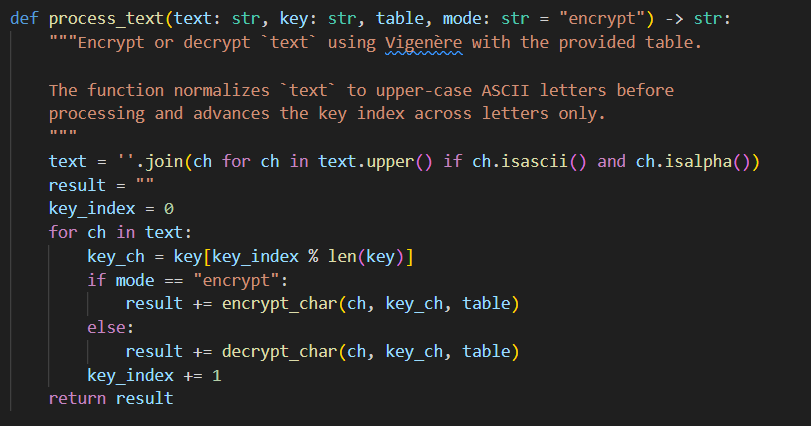
\includegraphics[width=\textwidth]{Recursos/vigenere.png}
	\caption{Cifragem e Decifragem com Vigenère.}
	\label{fig:vigenere}
\end{figure}

%---------------------------------------------------------------------------------------------------------------------------
\newpage
\subsection{PlayFair}
Implementou‑se uma ferramenta para cifragem e decifragem de ficheiros usando a cifra de Playfair com uma tabela 5×5 carregada através de um ficheiro.
A rotina interna \texttt{read\_board\_from\_file} lê e valida a tabela (linhas de letras; caracteres não‑alfabéticos são ignorados), mapeia 'J' para 'I' e, se necessário,
preenche os restantes caracteres A..Z (sem J). A normalização do texto é feita por \texttt{fix\_message}: conserva apenas letras ASCII, converte para maiúsculas,
insere 'X' entre letras duplicadas num digrafo e adiciona 'X' se necessário para obter comprimento par. O par (digrafo) é transformado por \texttt{process\_pair}
segundo as regras de Playfair (mesma linha → deslocamento horizontal; mesma coluna → deslocamento vertical; caso rectangular → troca de colunas).
As funções \texttt{encrypt\_text}/\texttt{decrypt\_text} aplicam o processamento ao texto; \texttt{encrypt\_file}/\texttt{decrypt\_file} leem/escrevem
ficheiros de texto usando o caminho da board como \texttt{key}. Em caso de ficheiro de board inexistente são lançadas exceções apropriadas.\\

\begin{figure}[H]
	\centering
	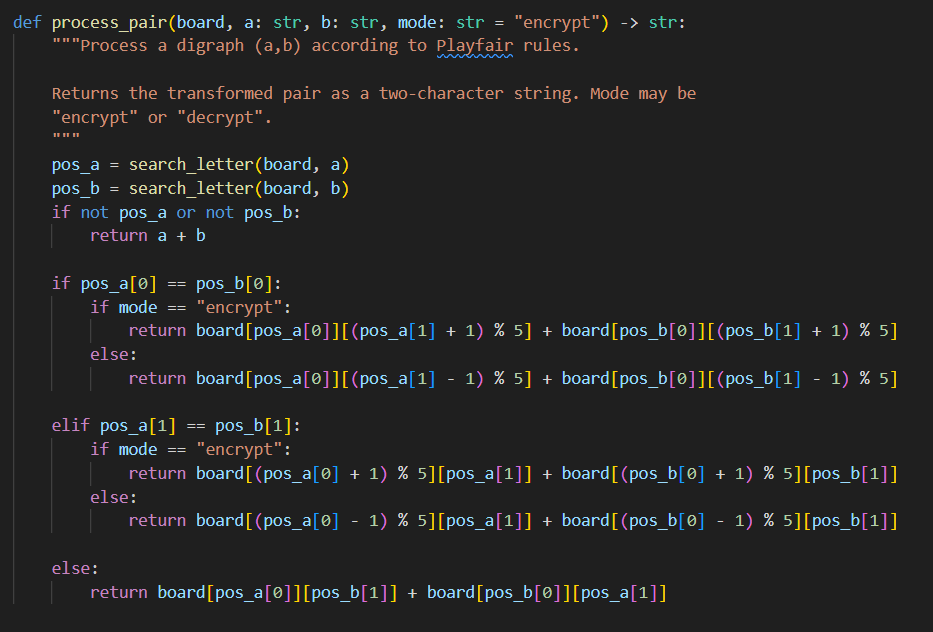
\includegraphics[width=\textwidth]{Recursos/playfair.png}
	\caption{Cifragem e Decifragem com PlayFair.}
	\label{fig:playfair}
\end{figure}

%---------------------------------------------------------------------------------------------------------------------------
\newpage
\subsection{Testes e Resultados}

%---------------------------------------------------------------------------------------------------------------------------
\newpage
\section{Conclusão}\label{con}
O desenvolvimento desta aplicação permitiu explorar conceitos fundamentais sobre cifras simétricas.
Apesar de alguns desafios encontrados, foi possível implementar as
cifras solicitadas e configurar uma interface centralizada para facilitar a utilização das mesmas.
Durante este processo, foram revistos conceitos previamente estudados na licenciatura de Engenharia Informática.
%---------------------------------------------------------------------------------------------------------------------------

\newpage
\renewcommand{\refname}{Bibliografia} % Para artigos
\renewcommand{\bibname}{Bibliografia} % Para livros e relatórios
\addcontentsline{toc}{section}{Bibliografia} % Adiciona a Bibliografia ao índice
\printbibliography

\end{document}
